\section{Zadání}

\textbf{Zadání č. 10}

\noindent \textbf{Model \enquote{Hmota na vozíku}}

\begin{enumerate}
    \item Pro daný systém sestavte
    
    \begin{enumerate}[label=\alph*)]
        \item model pomocí \textit{SimMechanics};
        \item model pomocí diferenciálních rovnic (odvoďte Newton-Eulerovou metodou);
        \item linearizovaný model v Simulinku pomocí bloku StateSpace.
    \end{enumerate}
    
    \item Porovnejte výsledky všech tří metod pro různé počáteční podmínky.
    \item Simulujte chování systému, pokud na něho bude působit síla o velikosti 10 N ve směru vektoru \textit{u} po dobu 10 sekund.
    \item Vykreslete frekvenční charakteristiku systému, jestliže vstupem je působící síla a výstupem poloha hmoty \textit{m}.
    \item Určete alespoň 1 konfiguraci senzorů polohy nebo rychlosti takovou, že systém bude:
    
    \begin{enumerate}[label=\alph*)]
        \item pozorovatelný;
        \item nepozorovatelný.
    \end{enumerate}
\end{enumerate}

Zadané hodnoty: \( m = 10 \: kg \), \( M = 2 \: kg \), \( l_{10} = 1 \: m \), \( k = 5 \), \( b = 0.7 \).

\begin{figure}[htbp]
	\centering
	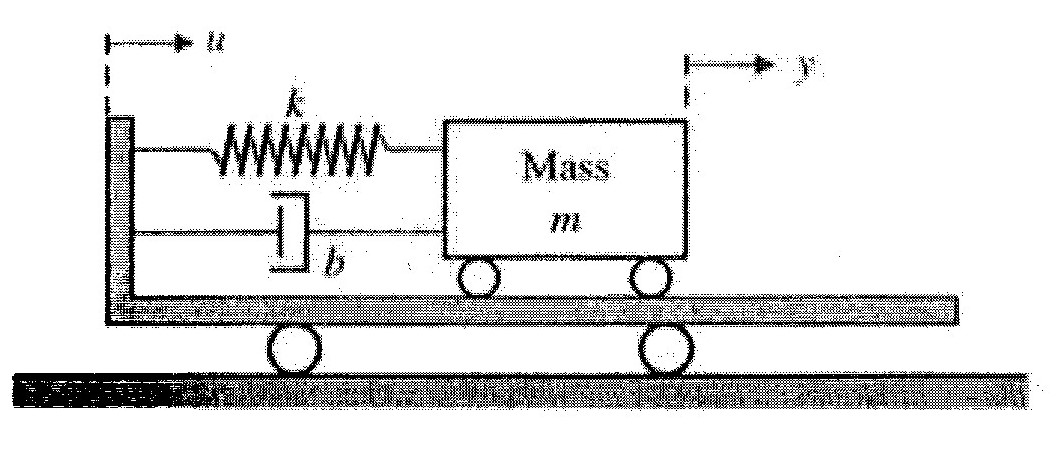
\includegraphics[scale=1]{img/model.jpg}
	\caption{Zadaný systém k nasimulování}
\end{figure}
\FloatBarrier
